\section{Tool Implementation}

\ctVerif is an open-source implementation of the constant-time verifier we
described earlier in \secref{body}. \figref{ct-verif-flow} illustrates the
tool flow from top to bottom. To prove constant-time security, a C function is
instantiated in a proof harness that declares public inputs (and outputs). Then,
the function alongside harness are compiled down to \codetext{llvm} bitcode. The
bitcodes are linked together and and then converted to \emph{Boogie Programming
Language} (\codetext{.bpl}). Compilation down to \codetext{.bpl} is automated
through \emph{SMACK}\cite{smack}, but it is possible to customize the flow if
needed and only rely on the the \codetext{bitcode} to \codetext{bpl} conversion
of SMACK.

The linked \codetext{bpl} files is then fed to \emph{BAM! BAM! Boogieman} which
performs the key task of generating the self-product (see \secref{body}), and
finally the self-product---which contains assertions and assumptions---is
given to \emph{Boogie}\cite{boogie} to verify safety of the self-product.


\begin{figure}[h]
    \centering
    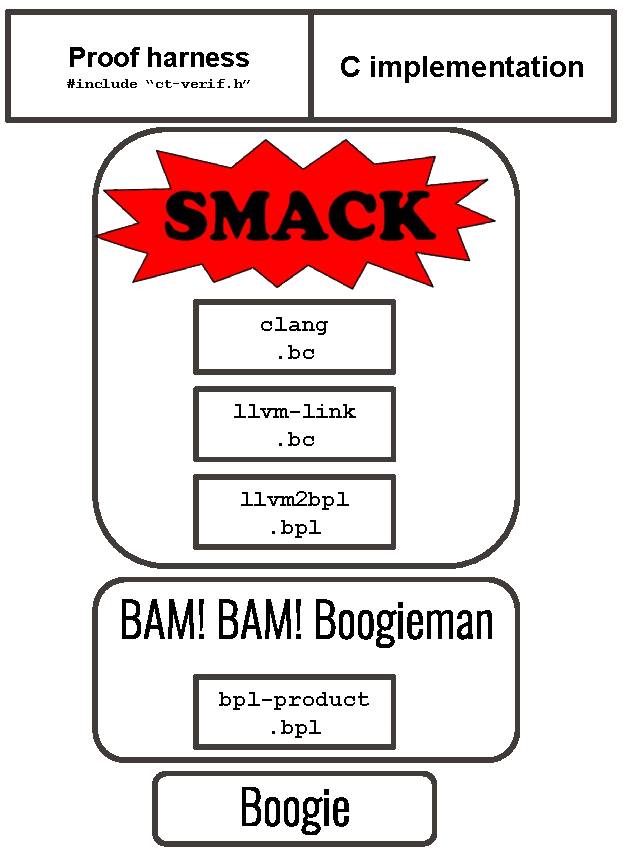
\includegraphics[width=\textwidth]{figs/ct-verif-flow.pdf}
    \caption{\ctVerif tool flow}
    \label{fig:ct-verif-flow}
\end{figure}